\chapter{Lecture 33 - The Finite Element Method, Galerkin Method and Weak Form}
\label{ch:lec33n}
\section{Objectives}
The objectives of this lecture are to:
\begin{itemize}
\item Describe the Method of Weighted Residuals to approximately solve a simple ODE.
\item Motivate and derive a Weak Formulation of the example problem.
\end{itemize}
\setcounter{lstannotation}{0}

\section{Example BVP}
Consider the following boundary value problem:
\begin{equation*}
\frac{d^2u}{dx^2}-u = -x, \ \ \ 0 < x < 1 
\end{equation*}
with homogeneous Dirichlet boundary conditions: $u(0)=u(1) = 0$.

\newthought{This is a} second-order, linear, non-homogeneous, equation with constant coefficients.  The complementary solution is: $u_c(x) = c_1\cosh{(x)}+c_2\sinh{(x)}$.  Using the method of undetermined coefficients, one can show that a particular solution is: $u_p = x$.  Combining the two gives us the general solution: $u(x) = u_c + u_p = x + c_1\cosh{(x)}+c_2\sinh{(x)}$. Applying boundary conditions gives us the solution:

\begin{equation}
u(x) = x - \frac{\sinh{(x)}}{\sinh{(1)}}
\label{eq:lec33n-ex-analytic}
\end{equation}
which is plotted in Figure \ref{fig:lec33n-ex1-exact}.
\begin{marginfigure}
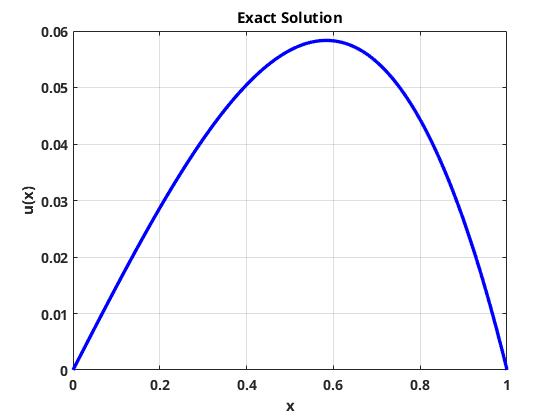
\includegraphics{lec33n-ex1-exact.png}
\caption{Exact solution of the example BVP.}
\label{fig:lec33n-ex1-exact}
\end{marginfigure}

\section{Method of Weighted Residuals}
In the past few lectures, we have explored a couple of different ways to approximately solve this problem.  All of them, in one way or another, have been based on a discrete approximation of the differential operator.  Today we will explore a method that takes a completely different approach.

\vspace{0.25cm}

\noindent\textbf{Step \#1:} Select a \emph{trial function} to represent the approximate solution; we will denote this as $\tilde{u}$.  For this problem, we select the trial function given in Equation \ref{eq:lec33n-ex1-trial-function}.  
\begin{equation}
\tilde{u}=ax(1-x)
\label{eq:lec33n-ex1-trial-function}
\end{equation}
where $a$ is a yet-to-be-determined parameter.\marginnote{Look again at the exact solution and mentally sketch a parabola to approximate $\tilde{u}$.  The goal will be to pick $a$, which relates to the maximum height of the parabola, such that $\tilde{u}$ is, in some sense, as close as possible to $u(x)$.}  The exact form of the trial function is up to you as the modeler but there are some attributes that an effective trial function should have, specifically:
\begin{enumerate}
\item The trial function used in an $n$-th order equation should have $n$ non-zero derivatives; and
\item the trial function should satisfy any Dirichlet boundary conditions.
\end{enumerate} 
Not coincidentally, the trial function given in Equation \ref{eq:lec33n-ex1-trial-function} satisfies those requirements for the given boundary value problem.

\vspace{0.25cm}

\noindent\textbf{Step \#2:} Compute the residual.  By \emph{residual}, we mean that we arrange the governing equation so all of the terms are on one side of the equation and we insert our trial function as the tentative solution as shown below:

\begin{align*}
R &= \frac{d^2\tilde{u}}{dx^2}-\tilde{u}+x \\
  &=-2a - ax(1-x) + x \\
\end{align*}

If we happened to  pick the exact solution as the trial function, the residual would be zero.  Since the exact solution involves the hyperbolic sine function, we cannot expect our 2\textsuperscript{nd}-order polynomial trial function to yield a zero residual.\sidenote{Recall that $\sinh{(x)} = \frac{e^{x}-e^{-x}}{2}$ and that exponentials are, essentially, infinite-order polynomials.  No finite-order polynomial can represent the exact solution.}

\newthought{As one might expect}, we will want to minimize the residual and this begs the question of how, exactly, we are to go about measuring the \emph{size} of the residual.  This brings us to the next step in the process.


\vspace{0.25cm}

\noindent\textbf{Step \#3:} Select a \emph{test function}, $w$, to serve as a weight for the residual.  The basic idea is that we will measure the size of the residual by taking the inner product of the residual and the weight function:
\begin{equation*}
\left(w,R\right) = \int_{a}^{b} wR\ dx
\end{equation*}

Among the several choices available for the weight function, we will describe three:
\begin{enumerate}
\item Set the weight function equal to the dereivative of the residual with respect to the unknown parameter $a$.  Specifically: $w=\frac{dR}{da} = -2 - x(1-x^2)$.  This is equivalent to what we did back in Lecture 13 of this text when we used Least Squares curve fitting except, in this case, we only have one equation.

\item Use the Dirac delta function, $w = \delta(x-x_0)$.\marginnote{\textbf{Note:} As any pedant worth his pounds in salt will quickly point out, the ``Dirac delta function'' is not a function in the usual sense but technically is a \emph{generalized function}. You should think of it in the same way you consider symbols such as $\infty$ to represent the somewhat abstract concept of infinity.  Whereas one might consider $\infty$ to represent a number that can increase without bound so that may be arbitrarily large, $\delta(x)$ is a ``function'' where $\delta(0)=\infty$ and $\delta(a)=0$ if $a\ne 0$.  The relevant property of $\delta(x)$ is when it is used in an integral where, if $a\le x_1 \le b$, then: $\int_{a}^{b} f(x)\delta{(x-x_1)} \ dx = f(x_1)$ if $x_1 \in [a,b]$.  If $x_1 \not\in [a,b]$, then $\int_{a}^{b} f(x) \delta{(x-x_1)} \ dx = 0$.}  This is known as the \emph{Colocation method}.  From the properties of the Dirac delta function, $\int_{a}^{b} \delta{(x-x_1)}R(x) \ dx = R(x_1)$, where, $x_1 \in [a,b]$, is known as a colocation point.   

\item Set the weight function equal to the derivative of the trial function with respect to the unknown parameter, $a$, so that: $w = \frac{d\tilde{u}}{da} = x(1-x)$. This is called the Galerkin method.\sidenote{Named after Boris Galerkin who was a Russian engineer and mathematician.  Interestingly, he wrote his first published paper while an inmate in the ``Kresty'' prison.}
\end{enumerate}

There are pros and cons to each of these approaches, a detailed discussion of which is beyond the scope of this text.  For reasons that will be discussed later, we will choose to use the Galerkin method for this example.

\vspace{0.25cm}

\noindent\textbf{Step \#4:} Minimize the weighted residual over the interval.  In particular, we will solve for $a$ such that:
\begin{equation*}
\left(w,R\right)=\int_{0}^{1} x(1-x)\left[-2a - ax(1-x) + x\right] \ dx = 0
\end{equation*}
In so doing, we will then, in a sense, have the value of $a$ such that $\tilde{u(x)}$ best represents the exact solution.  MATLAB code to carry out this task is shown in the listing below.
\marginnote{

\vspace{4.5cm}

\noindent\ref{lst:ann33n-1} Alternatively, you can use any other appropriate tool for solving a non-linear equation.

}
\begin{lstlisting}[style=myMatlab,name=lec33n-ex1]
clear
clc
close 'all'

u_exact = @(x) x - sinh(x)/sinh(1);
u_trial = @(x,a) a.*(x - x.^2);
Resid = @(x,a) -2*a - a.*x + a.*(x.^2) + x;
Weight_Galerkin = @(x) x.*(1-x);

F = @(a) integral(@(x) Weight_Galerkin(x).*Resid(x,a),0,1);

a = fzero(F,1); /*!\annotation{lst:ann33n-1}!*/
fprintf('a = %12.11f \n',a);
\end{lstlisting}
\begin{marginfigure}
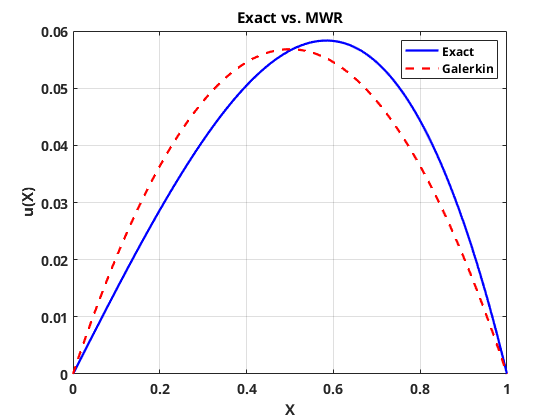
\includegraphics{lec33n-ex1-galerkin.png}
\caption{Approximate solution using the Galerkin method.}
\label{fig:lec33n-ex1-galerkin}
\end{marginfigure}
For this example problem, $a = 0.227272727$ is the resulting parameter value.  The approximate solution can be compared with the exact solution in Figure \ref{fig:lec33n-ex1-galerkin}.  

\newthought{In the likely} event that one would like to obtain a more accurate approximation to the solution, the following approaches are available:

\begin{enumerate}
\item Choose a more complex trial and test function.  For example, one might choose higher-order polynomials or even trigonometric functions. This is the approach taken in Chebyshev and Fourier spectral methods as described in, for example, the amazing textbook by Boyd.\cite{boyd}  This is often referred to as $p$-refinement, where $p$ is meant to represent the order of polynomial used for the trial and test functions.

\item Subdivide the domain with trial and test functions defined on each of the sub-domains.  This approach is referred to as $h$-refinement.  Finite Element Methods (FEM), that will be introduced in the next lecture take, this approach.  

\item Do a combination of \#1 and \#2 above.  This is sometimes called $hp$-refinement.
\end{enumerate}  
All of these approaches will be illustrated in the next lecture on FEM.

\section{Weak Formulation}
Before we finish this lecture, there is one more detail that I would like to address.  There is at least one drawback to the method of weighted residuals as we have described it so far.  That is that the trial function really needs to have two non-zero derivatives to be useful for the second-order differential operator.  We could not, therefore, choose piecewise-linear functions for our trial or test functions if we pursued an $h$-refinement approach.  The problem is that we \emph{really want} to choose piecewise-linear functions.  They're so simple to use and, with enough pieces, they can describe pretty much any function with arbitrary precision.  

\newthought{On the surface} it would seem that there is nothing to be done about our little problem.  It is, after all, a second-order differential operator and we can't change that, right?  Well, actually we can.  That is what the weak form is all about.  Let us re-visit the method of weighted residuals in, what we will now call, its ``strong form'':

\marginnote{

\vspace{4.0cm}

\noindent\textbf{Note:} Notice that the first term on the left-hand-side of the last line involves derivative of the trial function at the boundary. 
}
\begin{align*}
\int_{0}^{1} w \left(\frac{d^2 \tilde{u}}{dx^2}-\tilde{u}+x \right) \ dx &= 0 \\
\underbrace{\int_{0}^{1} w \frac{d^2 \tilde{u}}{dx^2} \ dx}_{\text{integrate by parts}} - \int_{0}^{1} w \tilde{u} \ dx + \int_{0}^{1}wx \ dx &= 0 \\
w \frac{d\tilde{u}}{dx}\Bigl|_0^1 - \int_{0}^{1}\frac{dw}{dx}\frac{d\tilde{u}}{dx}\ dx - \int_{0}^{1} w \tilde{u} \ dx + \int_{0}^{1}wx \ dx &= 0 \\
\end{align*}
The last line is what we call the ``weak form'' of the governing equation.  Notice that now both the trial and test function need have only one non-zero derivative.  We can solve this to find $a$.  This process is shown in the MATLAB listing below.

\begin{lstlisting}[style=myMatlab,name=lec33n-weak-form]
%% Weak Form
W = @(x) x - x.^2;
Ut = @(x,a) a.*(x - x.^2);
dW_dx = @(x) 1 - 2*x;
dUt_dx = @(x,a) a.*(1-2*x);

Weak_Form = @(a) W(1)*dUt_dx(1,a) - W(0)*dUt_dx(0,a) - ... 
    integral(@(x) dW_dx(x).*dUt_dx(x,a),0,1) - ...
    integral(@(x) W(x).*Ut(x,a),0,1) + ...
    integral(@(x) W(x).*x,0,1);

a_weak = fzero(Weak_Form,1);
\end{lstlisting}
The resut is: \lstinline[style=myMatlab]{a_week} = 0.22727272727, just as with the strong form.

\newthought{The fact that} the trial and test functions can now be piecewise linear is not the only advantage of the weak form.  Another advantage lies with the inclusion of the derivative of the trial function at the boundary in our formulation. Recall that we chose the trial function in part for the fact that it satisfied the Dirichlet boundary conditions.  Satisfying the type-1 boundary condition is, in this sense, ``essential'' and, for some expositions on FEM, is why such boundary conditions are often referred to as \emph{essential boundary conditions.}  In the weak form, we also expose type-2 boundary conditions within the residual that we are minimizing.  It is here where we now have the opportunity to specify a type-2 boundary condition directly within the formulation.  In the literature, type-2 boundary conditions are often referred to as \emph{natural boundary conditions} and it is in this sense that they appear ``naturally'' within the formulation. 
 


